\documentclass[tikz,border=6mm]{standalone}
\usepackage{tikz}
\usepackage{xcolor}
\usetikzlibrary{arrows.meta,calc,decorations.pathmorphing,decorations.markings,shapes.geometric,positioning,backgrounds,fit,shadings,patterns}
\definecolor{substblue}{RGB}{70,130,180}
\definecolor{procamber}{RGB}{180,110,30}
\definecolor{feltgreen}{RGB}{0,110,55}
\definecolor{bgcream}{RGB}{252,248,240}
\definecolor{atomblue}{RGB}{100,160,210}
\definecolor{emphred}{RGB}{160,40,40}
\definecolor{panelborder}{RGB}{180,170,155}

\begin{document}
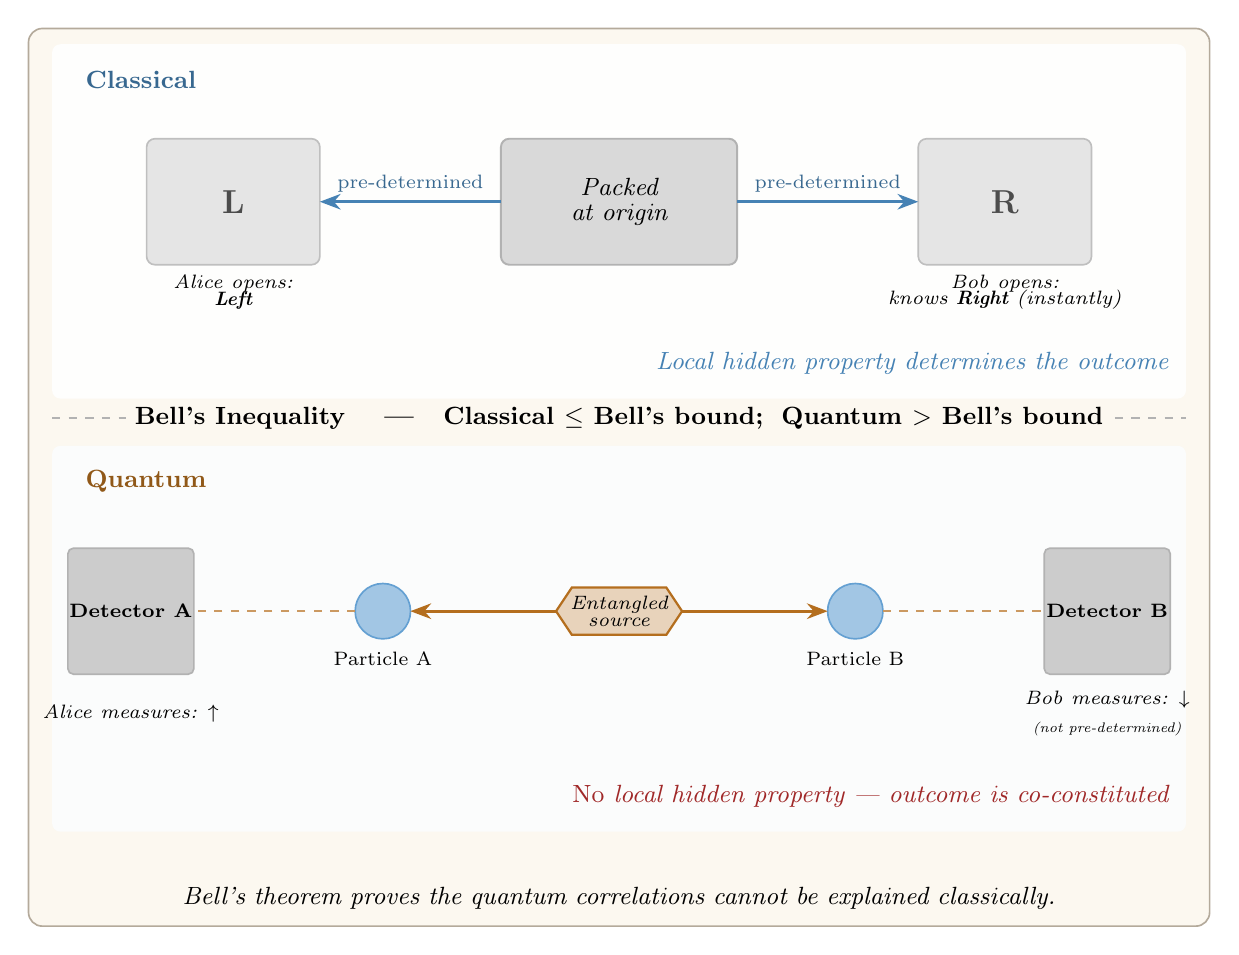
\begin{tikzpicture}[>=Stealth,font=\small]

%% ── overall background ───────────────────────────────────────────────────────
\fill[bgcream,rounded corners=5pt] (-0.5,-6.2) rectangle (14.5,5.2);
\draw[panelborder,rounded corners=5pt,line width=0.6pt]
  (-0.5,-6.2) rectangle (14.5,5.2);

%% ════════════════════════════════════════════════════════════════════════════
%%  UPPER ROW — Classical Correlation
%% ════════════════════════════════════════════════════════════════════════════
\fill[bgcream!95!substblue!10,rounded corners=3pt]
  (-0.2,0.5) rectangle (14.2,5.0);

%% row label
\node[font=\small\bfseries,substblue!80!black,anchor=west]
  at (0.1,4.55) {Classical};

%% source box
\fill[gray!30,rounded corners=3pt] (5.5,2.2) rectangle (8.5,3.8);
\draw[gray!60,rounded corners=3pt,line width=0.7pt] (5.5,2.2) rectangle (8.5,3.8);
\node[align=center,font=\small\itshape] at (7.0,3.0) {Packed\\[-2pt]at origin};

%% left glove box
\fill[gray!20,rounded corners=3pt] (1.0,2.2) rectangle (3.2,3.8);
\draw[gray!50,rounded corners=3pt,line width=0.6pt] (1.0,2.2) rectangle (3.2,3.8);
\node[font=\large\bfseries,gray!60!black] at (2.1,3.0) {L};

%% right glove box
\fill[gray!20,rounded corners=3pt] (10.8,2.2) rectangle (13.0,3.8);
\draw[gray!50,rounded corners=3pt,line width=0.6pt] (10.8,2.2) rectangle (13.0,3.8);
\node[font=\large\bfseries,gray!60!black] at (11.9,3.0) {R};

%% arrows source → gloves
\draw[->,substblue,line width=1.0pt] (5.5,3.0) -- (3.2,3.0);
\node[above,font=\scriptsize,substblue!80!black] at (4.35,3.0) {pre-determined};
\draw[->,substblue,line width=1.0pt] (8.5,3.0) -- (10.8,3.0);
\node[above,font=\scriptsize,substblue!80!black] at (9.65,3.0) {pre-determined};

%% sub-labels
\node[font=\scriptsize\itshape,align=center] at (2.1,1.85)
  {Alice opens:\\[-2pt]\textbf{Left}};
\node[font=\scriptsize\itshape,align=center] at (11.9,1.85)
  {Bob opens:\\[-2pt]knows \textbf{Right} (instantly)};

%% local hidden property note — placed below the row, clear of glove box
\node[font=\small\itshape,substblue,align=right,anchor=east] at (14.1,0.95)
  {\textcolor{substblue}{Local hidden property determines the outcome}};

%% ════════════════════════════════════════════════════════════════════════════
%%  DIVIDING LINE — Bell's Inequality
%% ════════════════════════════════════════════════════════════════════════════
\draw[gray!60,dashed,line width=0.8pt] (-0.2,0.25) -- (14.2,0.25);
\node[fill=bgcream,inner sep=3pt,font=\small\bfseries,align=center]
  at (7.0,0.25)
  {Bell's Inequality \quad|\quad
   Classical $\leq$ Bell's bound;\; Quantum $>$ Bell's bound};

%% ════════════════════════════════════════════════════════════════════════════
%%  LOWER ROW — Quantum Entanglement
%% ════════════════════════════════════════════════════════════════════════════
\fill[bgcream!85!atomblue!15,rounded corners=3pt]
  (-0.2,-5.0) rectangle (14.2,-0.1);

%% row label
\node[font=\small\bfseries,procamber!80!black,anchor=west]
  at (0.1,-0.55) {Quantum};

%% entangled source — star-burst diamond
\fill[procamber!30] (7.0,-2.5) -- (7.6,-2.5) -- (7.8,-2.2) -- (7.6,-1.9)
  -- (7.0,-1.9) -- (6.4,-1.9) -- (6.2,-2.2) -- (6.4,-2.5) -- cycle;
\draw[procamber,line width=0.8pt] (7.0,-2.5) -- (7.6,-2.5) -- (7.8,-2.2) -- (7.6,-1.9)
  -- (7.0,-1.9) -- (6.4,-1.9) -- (6.2,-2.2) -- (6.4,-2.5) -- cycle;
\node[font=\scriptsize\itshape,align=center] at (7.0,-2.2)
  {Entangled\\[-2pt]source};

%% particle A (left)
\fill[atomblue!60] (4.0,-2.2) circle (10pt);
\draw[atomblue,line width=0.6pt] (4.0,-2.2) circle (10pt);
\node[font=\scriptsize,align=center] at (4.0,-2.8) {Particle A};

%% particle B (right)
\fill[atomblue!60] (10.0,-2.2) circle (10pt);
\draw[atomblue,line width=0.6pt] (10.0,-2.2) circle (10pt);
\node[font=\scriptsize,align=center] at (10.0,-2.8) {Particle B};

%% curved arrows from source to particles
\draw[->,procamber,line width=1.0pt]
  (6.2,-2.2) to[out=180,in=0] (4.35,-2.2);
\draw[->,procamber,line width=1.0pt]
  (7.8,-2.2) to[out=0,in=180] (9.65,-2.2);

%% entanglement bond (dashed procamber line between particles)
\draw[procamber!70,dashed,line width=0.7pt] (3.65,-2.2) -- (1.0,-2.2);
\draw[procamber!70,dashed,line width=0.7pt] (10.35,-2.2) -- (13.0,-2.2);

%% detector A
\fill[gray!40,rounded corners=2pt] (0.0,-3.0) rectangle (1.6,-1.4);
\draw[gray!60,rounded corners=2pt,line width=0.6pt]
  (0.0,-3.0) rectangle (1.6,-1.4);
\node[font=\scriptsize\bfseries] at (0.8,-2.2) {Detector A};

%% detector B
\fill[gray!40,rounded corners=2pt] (12.4,-3.0) rectangle (14.0,-1.4);
\draw[gray!60,rounded corners=2pt,line width=0.6pt]
  (12.4,-3.0) rectangle (14.0,-1.4);
\node[font=\scriptsize\bfseries] at (13.2,-2.2) {Detector B};

%% measurement results
\node[font=\scriptsize\itshape,align=center] at (0.8,-3.5)
  {Alice measures: $\uparrow$};
\node[font=\scriptsize\itshape,align=center] at (13.2,-3.5)
  {Bob measures: $\downarrow$\\[2pt]
   \tiny\itshape(not pre-determined)};

%% no local hidden property — placed below the quantum row, clear of detector boxes
\node[font=\small\itshape,emphred,align=right,anchor=east] at (14.1,-4.55)
  {\textcolor{emphred}{\emph{No} local hidden property --- outcome is co-constituted}};

%% ── caption (inside extended bgcream, outside both panel backgrounds) ───────
\node[font=\small\itshape,text width=13cm,align=center]
  at (7.0,-5.85)
  {Bell's theorem proves the quantum correlations cannot be explained classically.};

\end{tikzpicture}
\end{document}
